\documentclass{beamer}

\usepackage{beamerthemeshadow}
\setbeamertemplate{navigation symbols}{}
\setbeamertemplate{caption}[numbered]

%load packages
\usepackage{graphicx} %provides support for graphics
\usepackage{epsfig}   %provides support for .eps
\usepackage{amsmath}  %some symbols / fonts


\begin{document}
\title{ASTR288P Lecture 11: \LaTeX} 
\author{Sean Griffin} 
\date{\today} 

\begin{frame}
\titlepage
\end{frame}

%\begin{frame}
%	\frametitle{Table of Contents}
%	\tableofcontents
%\end{frame} 


\section{Introduction} 
\begin{frame}
\frametitle{Introduction}
\begin{block}{Word Processors}
Word processors are typically WYSIWYG (what you see is what you get). 

User is in direct control of aesthetics of the document. 
\end{block}

\begin{block}{\LaTeX}
\LaTeX\ (pronounced ``lay-tech'' or ``lah-tech'') is a popular typesetting application used ubiquitously in physics and astronomy.

Documents are coded and compiled to produce the final document. 
\end{block}

\end{frame}


\begin{frame}
\frametitle{Introduction}
Why use \LaTeX? 
\begin{itemize}
	\item Powerful cross-referencing tools, bibliographies, automatic ToC generation
	\item Allows the author to focus on the content rather than the appearance
	\item Many useful packages for a variety of applications: 
	\begin{itemize}
		\item Hyperlinks (hyperref)
		\item Code insertion (listings)
		\item Automatic bibliography generation and formatting (BibTex)
	\end{itemize}
	\item Free
	\item Cross-platform (Windows, Linux, OS X)

\end{itemize}
\end{frame}


\section{Examples}
\begin{frame}[fragile]
\frametitle{Hello World Example}
\begin{verbatim}
\documentclass{article}
\title{ASTR288P Hello World Example}
\author{Sean Griffin}
\date{November 2017}
\begin{document}
   \maketitle
   Hello world!
\end{document}
\end{verbatim}
\end{frame}


\begin{frame}[fragile]
\frametitle{Verbatim Text}
Text enclosed inside \texttt{verbatim} environment 
is printed directly 
and all \LaTeX{} commands are ignored.
\begin{verbatim}
Text enclosed inside \texttt{verbatim} environment 
is printed directly 
and all \LaTeX{} commands are ignored.
\end{verbatim}

\end{frame}

\begin{frame}
\frametitle{beamer}
The \textbf{beamer} class is a popular \LaTeX\ class used for producing presentations and posters. 
There are many different styles (e.g. the lecture notes for Lectures 1 and 2 use the ``metropolis'' theme).
Can be tricky -- sometimes it's faster to just use Powerpoint but \textbf{beamer} produces very nice slides with cool \LaTeX\ functionality.
\end{frame}

\section{Environments}
\begin{frame}
Environments are delimited by \texttt{\textbackslash begin} and \texttt{\textbackslash end} tags.

There are many different environments:
\begin{center}
For example, this is a centered environment.
\end{center}

In \textbf{beamer}, each new slide is a \texttt{frame} environment. 

There are also \texttt{block} environments which allow us to emphasize certain things and help us format our presentation.
\end{frame}


\begin{frame}[fragile]
\frametitle{Labels and Referencing}
\begin{block}{Labels}
Inside certain environments (e.g. equation, figure, table, or even sections and subsections) we can give them labels that can be used to refer to the item later.	
As we add (e.g.) equations, the equation numbers are handled for us automatically. No need to keep track.
\end{block}
\begin{exampleblock}{Example}
\begin{verbatim}
\begin{equation}
\label{eq:fit_result}
\frac{dN}{dE} = F_0 \frac{E}{1~\mathrm{TeV}}^{-\Gamma}
\end{equation}
...
Now we can refer to it by referring to 
Equation \ref{eq:fit_result}.
\end{verbatim}

\end{exampleblock}

\end{frame}

\begin{frame}
\frametitle{Equations}
	\begin{equation}
		\label{eq:mass-enertgy}
		E = m c^2
	\end{equation}
	
	We can put some text here, and even refer to Equation \ref{eq:mass-enertgy}. 	
	\begin{eqnarray}
	F = m a\\
	\vec{F} = -G \frac{M m}{r^2}\hat{r}\notag\\
	\nabla \cdot E = \frac{\rho}{\epsilon_0 }
	\end{eqnarray}
\end{frame}

\begin{frame}
\frametitle{Tables}
\begin{table}
\centering
\begin{tabular}{cc|l|lr}
\hline\hline
5 & 5 & a & 12 & g\\
5 & 5 & a & 12 & g\\
word & another & another & another & another\\
a & b & c & d & e\\
\hline\hline
\end{tabular}
\caption{This is a table caption.}
\label{tab:example_table}
\end{table}
\end{frame}

\begin{frame}
\frametitle{Figures}

\begin{columns}
\begin{column}{0.5\textwidth}
\begin{block}{Columns in a Frame}
This is a block next to a figure; we did this using the \texttt{columns} environment.
\end{block}
\end{column}

\begin{column}{0.5\textwidth}
\begin{figure}
\centering
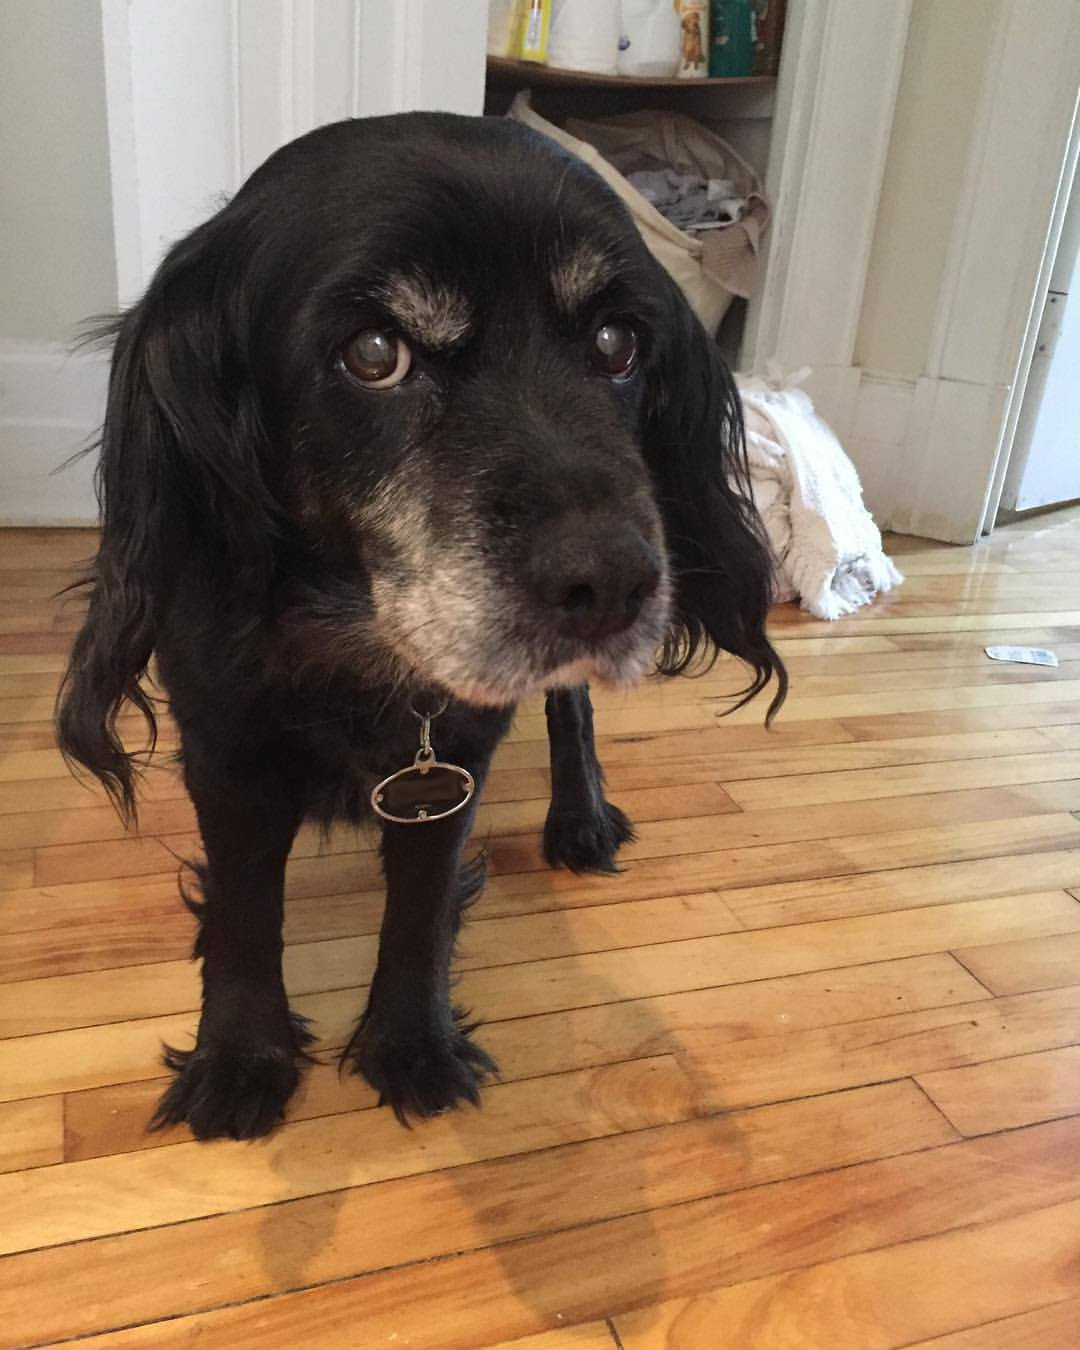
\includegraphics[width=0.5\textwidth]{figures/brittany}
\caption{This is a figure caption. 
Describe your plot, scale, axes, etc. in this text. 
Otherwise, look at the cute doggo.}
\label{fig:example_figure}
\end{figure}
\end{column}
\end{columns}
\end{frame}

\section{Compiling Latex Code}
\begin{frame}[fragile]
To view a completed \LaTeX\ document, you must compile the code. 
There are generally two ways to do this. 
You can use 
\begin{verbatim}
% latex document.tex
% dvipdf document.dvi
\end{verbatim}
or
\begin{verbatim}
% pdflatex document.tex
\end{verbatim}
which directly produces a PDF document. Depending on the packages you are using,  you might be required to use \texttt{pdflatex}.

To view our document, we can use the \texttt{evince} program, which is generally included with linux. 
\end{frame}

\section{Homework Assignment}
\begin{frame}
TBD
\end{frame}


\end{document}